\section{Architecture for DUMs Details}
\label{subsec:appendix_encoder}


% -------------------------------------------


% \subsection{Regularization constraints}

For all the architecture experiments we used the default training settings in \cref{subsec:appendix_training} and \cref{tab:appendix_default_hyper}.

\textbf{Bi-Lipschitz training details.} In the \textit{None} configuration, we removed the residual connection from the architecture for both the pretraining of the encoder and the joint training phase. In the \textit{Residual} configuration, we did not modify anything since both ResNet and WideResNet already use the residual connection. While for the \textit{bi-Lipschitz} configuration, we added the spectral normalization during both the pretraining and also joint training phase. Following the original method presented in \cite{due}, we used the same implementation and applied spectral normalization to the linear, convolution, and batch normalization layers. During the model selection, using the validation set results, we find that the best \textit{Lipschitz constant} $c$ for DUE is 4, and for NatPN is 5. For both the models the power iteration parameter is set to 1. For the toy dataset we use an encoder with 4 linear layers of 128 dimension each.

\begin{figure}[!htb]
    \centering
    \includegraphics[width=\textwidth]{sections/008_iclr2023/figures/bi_bar.pdf}
    \caption{Results OOD generalization and OOD detection results of DUMs with none, residual and bi-lipschitz \textbf{architecture constraints}. Bi-lipschitz and more specifically can improve OOD detection by mitigating feature collapse (see \cref{fig:bi_toy}) at the expense of degrading OOD generalization.}
    \label{fig:bi_bar_full}
\end{figure}

\begin{figure}[!htb]
    \centering
    \includegraphics[width=0.75\textwidth]{sections/008_iclr2023/figures/reconst.pdf}
    \caption{Results OOD generalization and OOD detection results of DUMs with reconstruction \textbf{architecture constraints}. Increasing the strength of the reconstruction factor $\lambda$ improves the OOD generalization only on the simpler MNIST/CMNIST datasets but fails for more complex datasets. }
    \label{fig:reconst_full}
\end{figure}

\textbf{Reconstruction training details.} The decoder reconstructs the input extracted from the last residual block of the encoder, before the pooling layer. During the pretraining phase, both the encoder and decoder are trained with the cross-entropy loss plus a MSE reconstruction term. During the joint training phase, we load the pretrained encoder and decoder, and joint train with the DUMs' respective loss plus the MSE reconstruction term. For the toy dataset we use an encoder with 4 linear layers of 128 dimension each.

\begin{figure}[!htb]
    \begin{subfigure}[b]{\textwidth}
        \centering
        \includegraphics[width=0.75\textwidth]{sections/008_iclr2023/figures/toy/blob2/bi.png}
        \caption{Bi-Lipschitz}
        \label{fig:bi_toy}
    \end{subfigure}
    \begin{subfigure}[b]{\textwidth}
        \centering
        \includegraphics[width=0.75\textwidth]{sections/008_iclr2023/figures/toy/blob2/rec.png}
        \caption{Reconstruction}
        \label{fig:rec_toy}
    \end{subfigure}
    \caption{\textbf{Regularization constraint toy dataset uncertainty boundaries with NatPN.} The two black dots represent the center of two different class of Gaussian data, sharing the same y-axis to trigger the \textit{feature collapse} phenomenon. The color represents the likelihood produced by the uncertainty head. Each row is a different setting, e.g. \textit{bi1.0} is the bi-Lipschitz constraint with the Lipschitz constant $c = 1$ and \textit{rec1.0} is the reconstruction term with $\lambda=1$. Each column is a different seed initialization. (top) \textbf{Bi-Lipschitz} experiment shows that the core encoder architecture constrained with a larger \textit{Lipschitz constant} in the last two rows behaves similar to the encoder constrained with only the residual connection (second row) showing that relaxing the spectral normalization constraint falls back to the residual connection, preventing the feature collapse. (bottom) \textbf{Reconstruction} experiment shows that it does not help to prevent feature collapse by itself. The core encoder architecture is not constrained with bi-Lipschitz. }
    \label{fig:toy}
\end{figure}

\begin{figure}[!htb]
    \begin{subfigure}[b]{\textwidth}
        \centering
        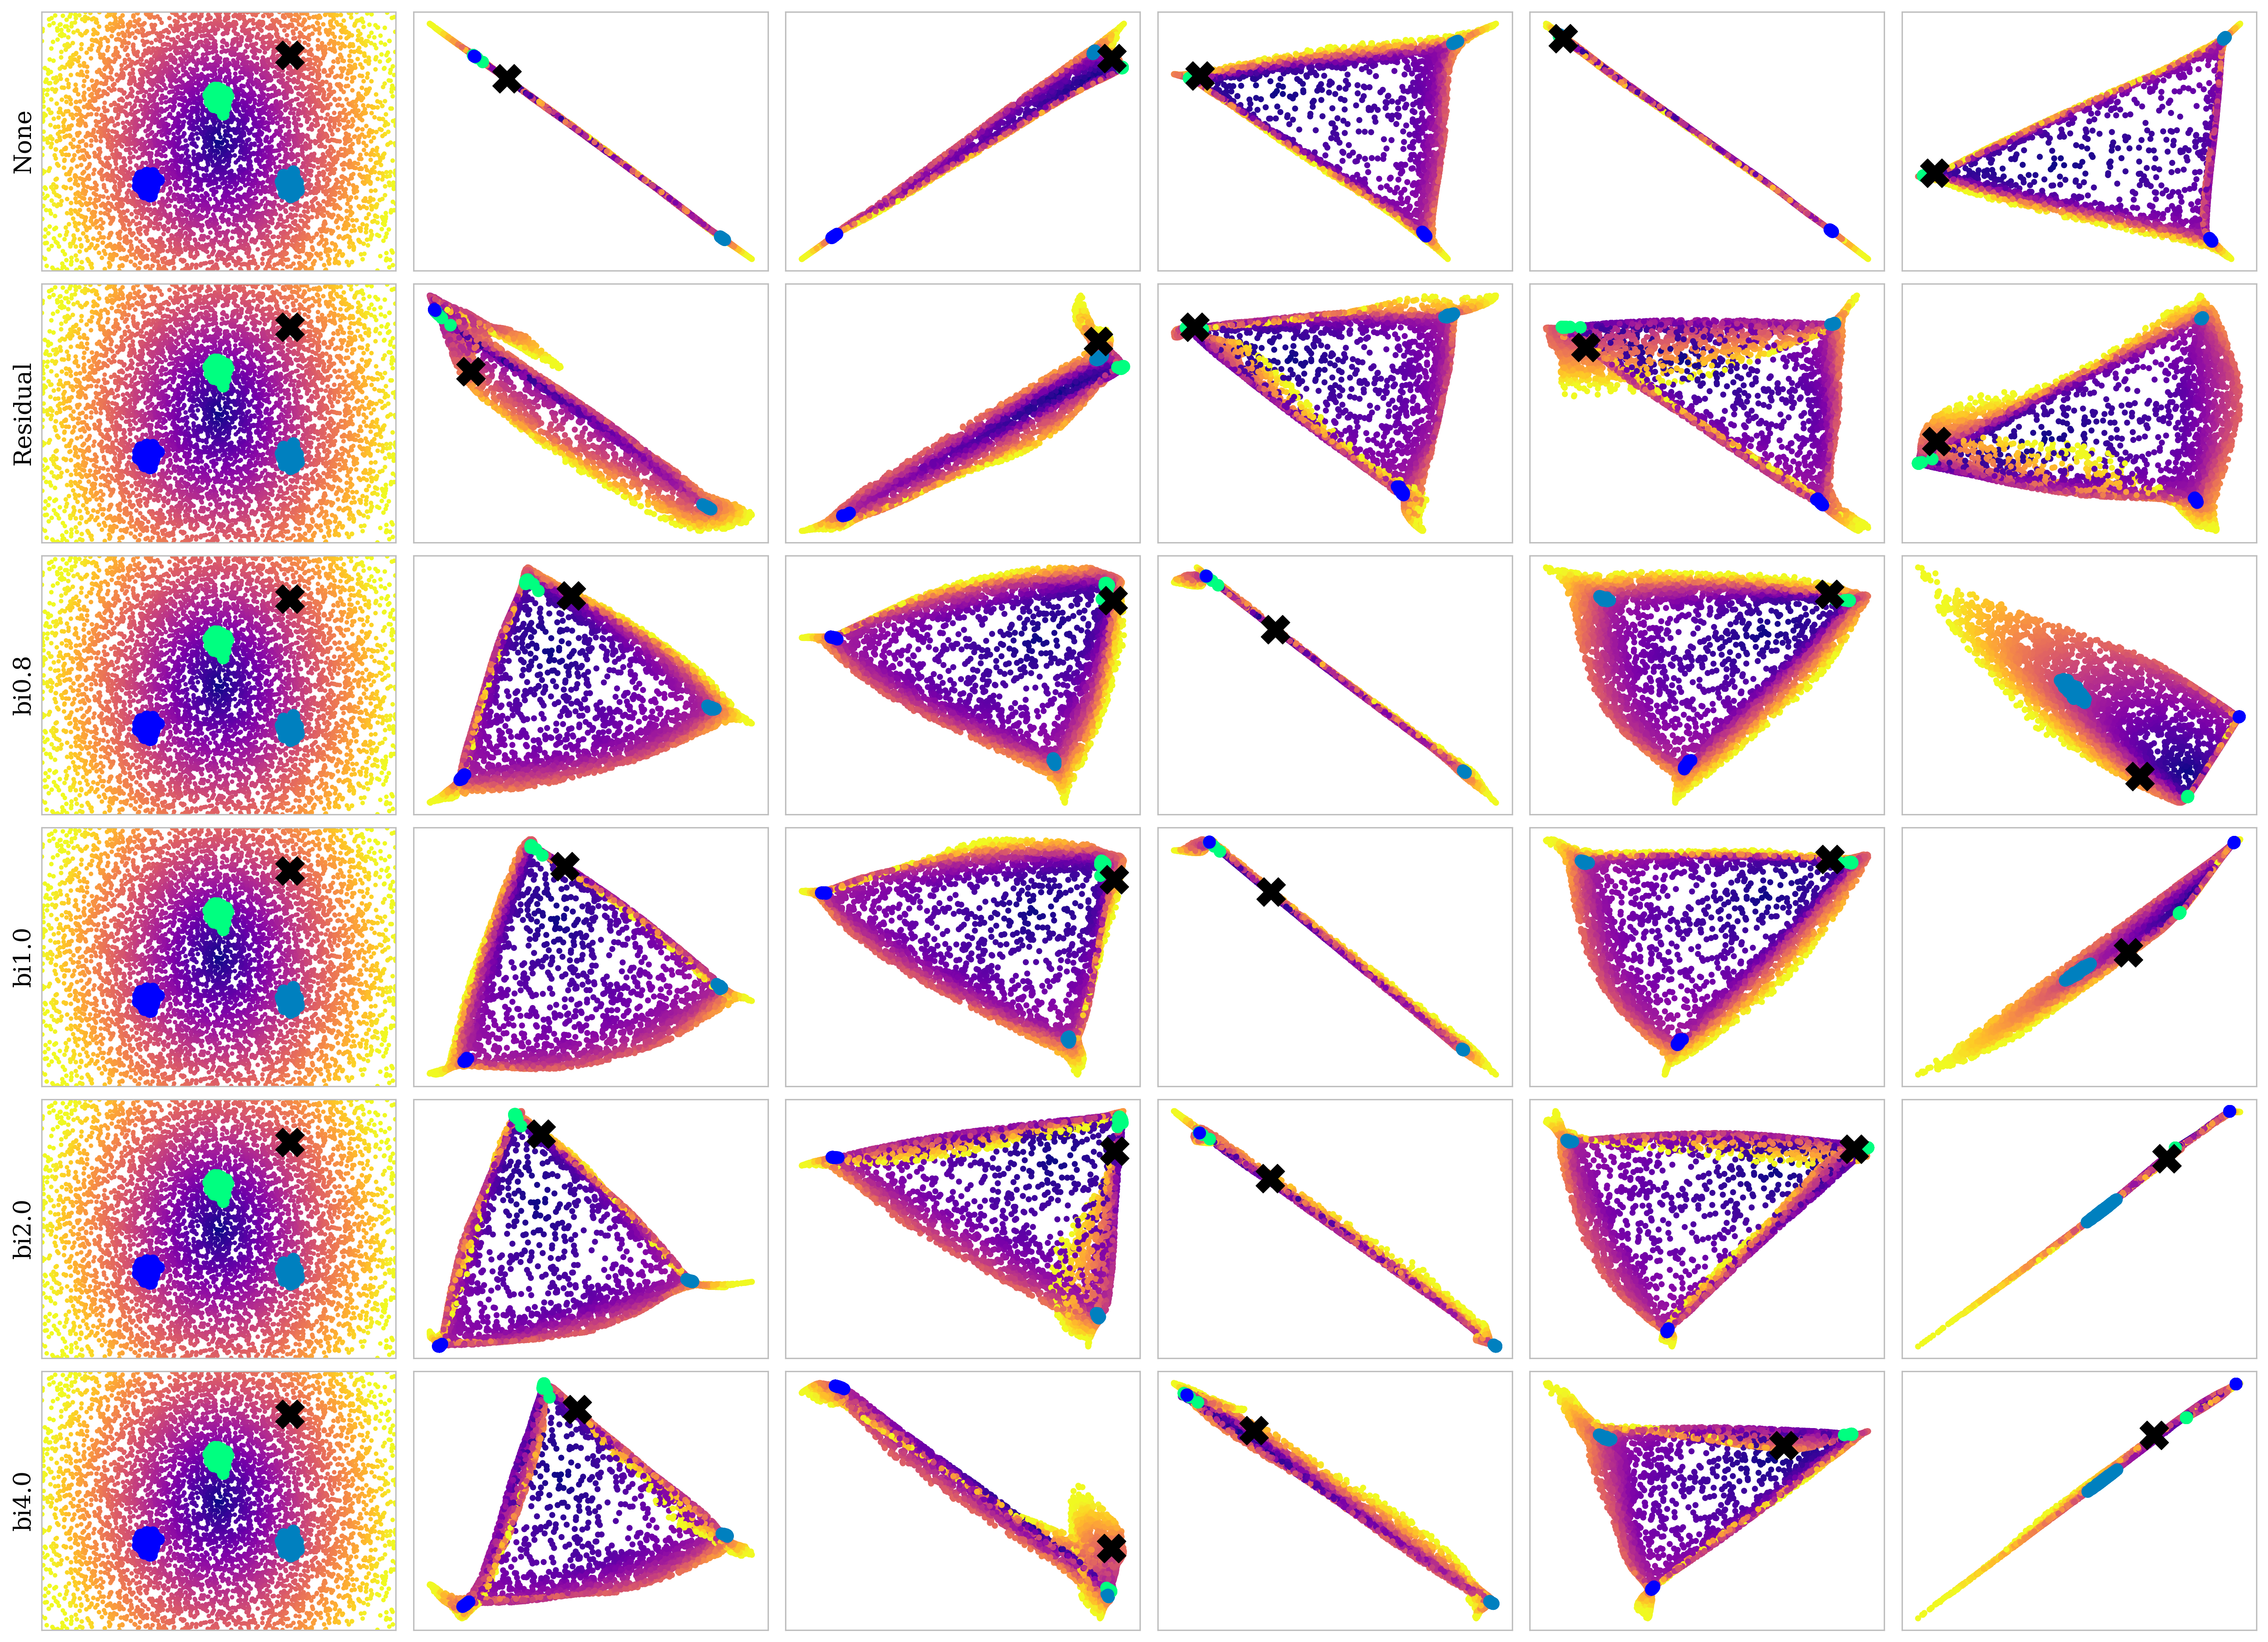
\includegraphics[width=0.8\textwidth]{sections/008_iclr2023/figures/toy/blob2/bi_collapse.png}
        \caption{Bi-Lipschitz}
        \label{fig:bi_toy_collapse}
    \end{subfigure}
    \begin{subfigure}[b]{\textwidth}
        \centering
        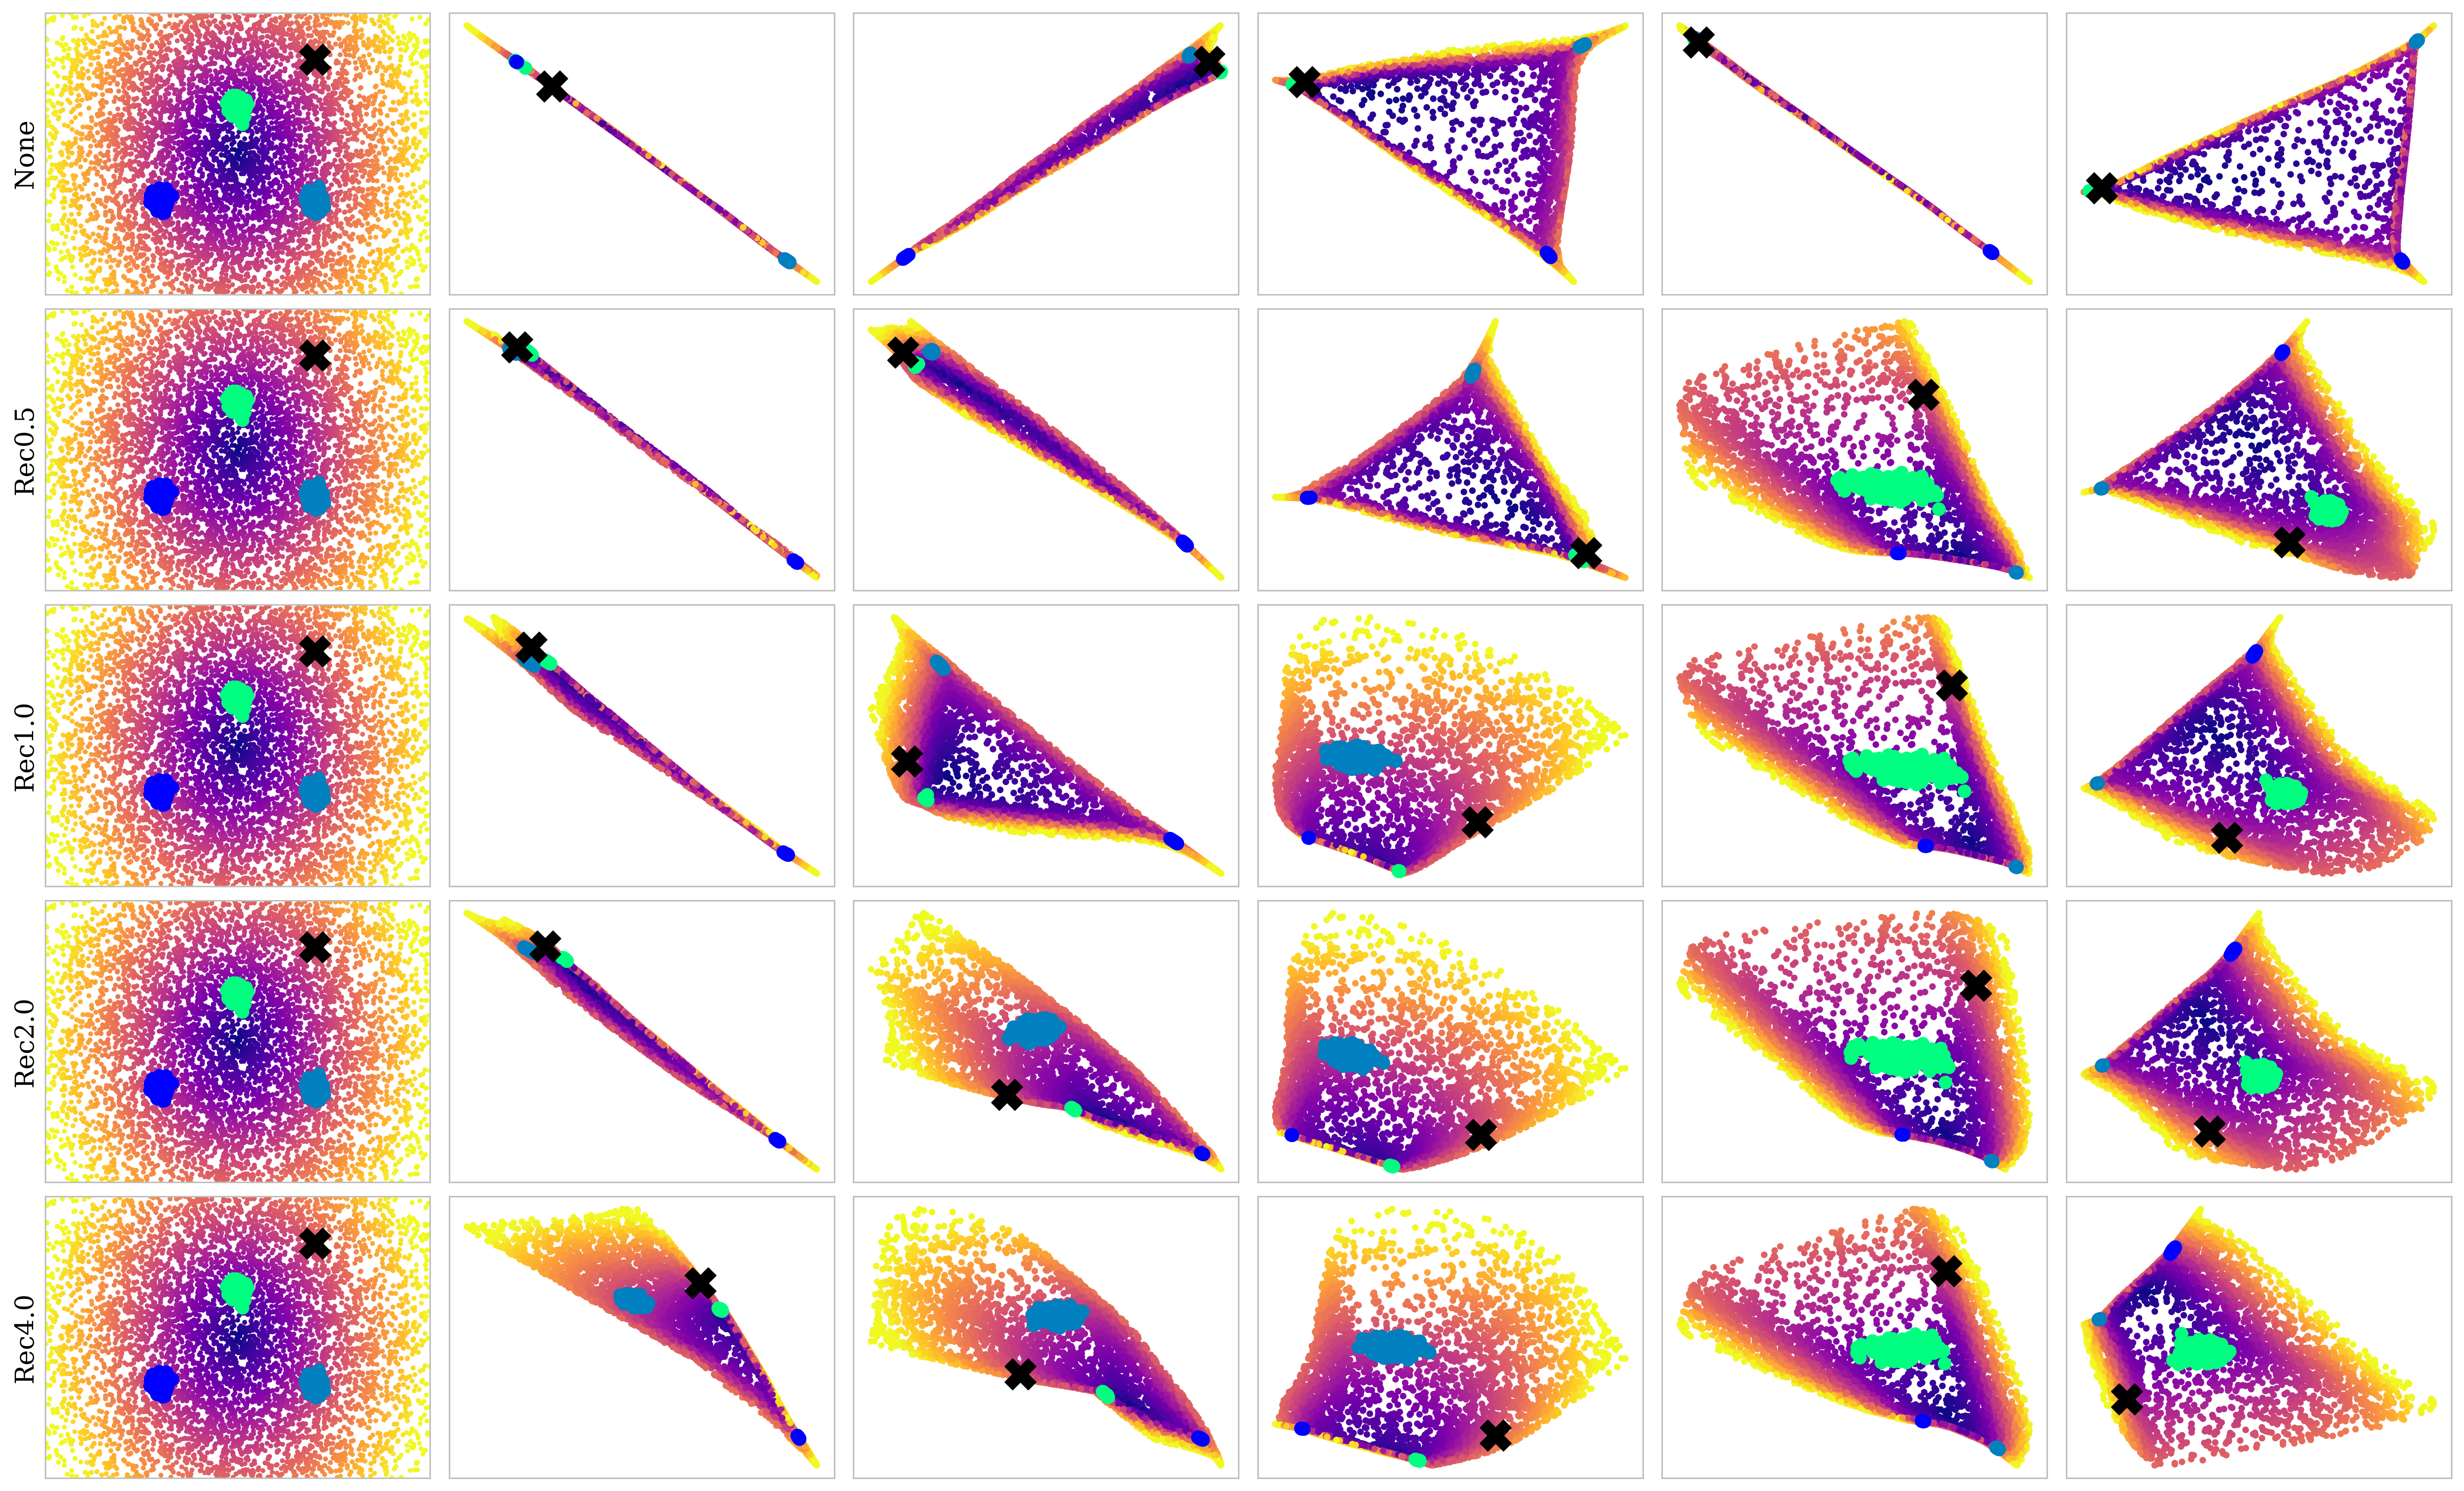
\includegraphics[width=0.8\textwidth]{sections/008_iclr2023/figures/toy/blob2/rec_collapse.png}
        \caption{Reconstruction}
        \label{fig:rec_toy_collapse}
    \end{subfigure}
    \caption{\textbf{Regularization constraint toy dataset feature collapse with NatPN.} Similarly to \citep{due}, we run the toy experiment where the first column represent two Gaussian class of data, sharing the same y-axis center to trigger the \textit{feature collapse} phenomenon, and a grid of unrelated point to simulate the space distorsion (colors are based on the Gaussian's generating distribution). 
    Each row is a different setting, e.g. \textit{bi1.0} is the bi-Lipschitz constraint with the Lipschitz constant $c = 1$ and \textit{rec1.0} is the reconstruction term with $\lambda=1$. Each column is a different seed initialization. Results are the same as \ref{fig:bi_toy}. Larger Lipschitz constant \textit{c} reverts back to the residual connection, and reconstruction regularization collapses the 2D dimension into one single dimension. }
    \label{fig:toy_collpase}
\end{figure}


% -----------------------------------


\begin{figure}[!htb]
    \centering
    \begin{subfigure}[b]{\textwidth}
        \includegraphics[width=\textwidth]{sections/008_iclr2023/figures/latent_ood_mnist.pdf}
        \caption{MNIST}
        \label{fig:latent_ood_mnist}
    \end{subfigure}
    \begin{subfigure}[b]{\textwidth}
        \includegraphics[width=\textwidth]{sections/008_iclr2023/figures/latent_ood_cifar10.pdf}
        \caption{CIFAR10}
        \label{fig:latent_ood_cifar10}
    \end{subfigure}
    \begin{subfigure}[b]{\textwidth}
        \includegraphics[width=\textwidth]{sections/008_iclr2023/figures/latent_ood_cifar100.pdf}
        \caption{CIFAR100}
        \label{fig:latent_ood_cifar100}
    \end{subfigure}
    \begin{subfigure}[b]{\textwidth}
        \includegraphics[width=\textwidth]{sections/008_iclr2023/figures/latent_ood_camelyon_id.pdf}
        \caption{Camelyon ID}
        \label{fig:latent_ood_camelyon}
    \end{subfigure}
    
    \caption{\textbf{Latent dimension OOD detection.} For each training dataset we show the uncertainty estimation results on the corresponding OOD dataset. NatPN encounters numerical instabilities with high latent dimension on Camelyon dataset, while DUE is less sensitive to the variation.}
    \label{fig:latent_ood}
\end{figure}


\begin{figure}[!htb]
    \centering
    \begin{subfigure}[b]{\textwidth}
        \includegraphics[width=\textwidth]{sections/008_iclr2023/figures/bi_bar_ood_mnist.pdf}
        \caption{MNIST}
        \label{fig:bi_bar_ood_mnist}
    \end{subfigure}
    \begin{subfigure}[b]{\textwidth}
        \includegraphics[width=\textwidth]{sections/008_iclr2023/figures/bi_bar_ood_cifar10.pdf}
        \caption{CIFAR10}
        \label{fig:bi_bar_ood_cifar10}
    \end{subfigure}
    \begin{subfigure}[b]{\textwidth}
        \includegraphics[width=\textwidth]{sections/008_iclr2023/figures/bi_bar_ood_cifar100.pdf}
        \caption{CIFAR100}
        \label{fig:bi_bar_ood_cifar100}
    \end{subfigure}
    \begin{subfigure}[b]{\textwidth}
        \includegraphics[width=\textwidth]{sections/008_iclr2023/figures/bi_bar_ood_camelyon_id.pdf}
        \caption{Camelyon ID}
        \label{fig:bi_bar_ood_camelyon}
    \end{subfigure}
    
    \caption{\textbf{Bi-lipschitz OOD detection.} For each training dataset we show the uncertainty estimation results on the corresponding OOD dataset. Bi-Lipschitz improvements are not consistent across different OOD datasets. }
    \label{fig:bi_ood}
\end{figure}


\begin{figure}[!htb]
    \centering
    \begin{subfigure}[b]{\textwidth}
        \includegraphics[width=\textwidth]{sections/008_iclr2023/figures/reconst_ood_mnist.pdf}
        \caption{MNIST}
        \label{fig:rec_ood_mnist}
    \end{subfigure}
    \begin{subfigure}[b]{\textwidth}
        \includegraphics[width=\textwidth]{sections/008_iclr2023/figures/reconst_ood_cifar10.pdf}
        \caption{CIFAR10}
        \label{fig:rec_ood_cifar10}
    \end{subfigure}
    \begin{subfigure}[b]{\textwidth}
        \includegraphics[width=\textwidth]{sections/008_iclr2023/figures/reconst_ood_cifar100.pdf}
        \caption{CIFAR100}
        \label{fig:rec_ood_cifar100}
    \end{subfigure}
    
    \caption{\textbf{Reconstruction regularization OOD detection.} Increasing the weight coefficient of the reconstruction loss term improved the OOD detection of NatPN in MNIST. However, we did not observe improvements on more complex datasets such as CIFAR.}
    \label{fig:rec_ood}
\end{figure}


\begin{figure}[!htb]
    \centering
    \includegraphics[width=0.8\linewidth]{sections/008_iclr2023/figures/reconst_samples.png}
    \caption{\textbf{Reconstruction regularization CIFAR samples.} (left) The original input (right) the reconstructed input after NatPN's joint training phase. The reconstruction discards detailed information compared to the original input. }
    \label{fig:rec_samples}
\end{figure}


\begin{table}[!htb]
\centering
\caption{\textbf{Encoder architecture OOD detection.} For each training dataset we show the uncertainty estimation results on the corresponding OOD dataset. We observe that new architectures (EfficientNet, Swin) have consistently better results. Interestingly, the transformer based model Swin, is not able to detect out-of-domain data, which should be easy in principle.}
\label{tab:encoder_architecture_ood}
\tiny
\begin{tabular}{lllccc}
    \toprule
    \textbf{Model} &\textbf{OOD Data} &\textbf{Architecture} &\textbf{OOD Alea. ($\uparrow$)} &\textbf{OOD Epis. ($\uparrow$)} &\textbf{OOD Pred. ($\uparrow$)} \\
    \midrule
    \multirow{20}{*}{NatPN} &\multirow{4}{*}{SVHN} &ResNet18 &\textbf{89.90 $\pm$ 1.22} &78.14 $\pm$ 3.13 &\textbf{89.90 $\pm$ 1.22} \\
    & &ResNet50 &89.34 $\pm$ 0.66 &92.02 $\pm$ 0.49 &89.34 $\pm$ 0.66 \\
    & &EfficientNet\_V2\_S &88.65 $\pm$ 0.68 &92.52 $\pm$ 0.60 &88.65 $\pm$ 0.68 \\
    & &Swin\_T &87.73 $\pm$ 1.36 &\textbf{94.17 $\pm$ 0.74} &87.73 $\pm$ 1.36 \\
    \cmidrule[0.1pt](lr){2-6}
    &\multirow{4}{*}{STL10} &ResNet18 &\textbf{90.99 $\pm$ 0.37} &83.90 $\pm$ 0.59 &\textbf{90.99 $\pm$ 0.37} \\
    & &ResNet50 &85.46 $\pm$ 0.50 &90.76 $\pm$ 0.31 &85.46 $\pm$ 0.50 \\
    & &EfficientNet\_V2\_S &88.68 $\pm$ 0.62 &91.11 $\pm$ 0.47 &88.68 $\pm$ 0.62 \\
    & &Swin\_T &85.44 $\pm$ 0.56 &\textbf{92.16 $\pm$ 0.40} &85.44 $\pm$ 0.56 \\
    \cmidrule[0.1pt](lr){2-6}
    &\multirow{4}{*}{CelebA} &ResNet18 &66.46 $\pm$ 3.48 &50.61 $\pm$ 2.14 &66.46 $\pm$ 3.48 \\
    & &ResNet50 &59.30 $\pm$ 3.77 &64.80 $\pm$ 2.15 &59.30 $\pm$ 3.77 \\
    & &EffNet\_V2\_S &\textbf{67.04 $\pm$ 1.74} &66.29 $\pm$ 1.45 &\textbf{67.04 $\pm$ 1.74} \\
    & &Swin\_T &63.60 $\pm$ 2.16 &\textbf{72.80 $\pm$ 1.00} &63.60 $\pm$ 2.16 \\
    \cmidrule[0.1pt](lr){2-6}
    &\multirow{4}{*}{Camelyon} &ResNet18 &90.09 $\pm$ 4.43 &96.28 $\pm$ 1.06 &90.09 $\pm$ 4.43 \\
    & &ResNet50 &90.64 $\pm$ 2.47 &97.82 $\pm$ 0.56 &90.64 $\pm$ 2.47 \\
    & &EfficientNet\_V2\_S &94.56 $\pm$ 0.79 &97.42 $\pm$ 0.44 &94.56 $\pm$ 0.79 \\
    & &Swin\_T &\textbf{95.43 $\pm$ 1.47} &\textbf{98.71 $\pm$ 0.50} &\textbf{95.43 $\pm$ 1.47} \\
    \cmidrule[0.1pt](lr){2-6}
    &\multirow{4}{*}{SVHN OODom.} &ResNet18 &\textbf{100.00 $\pm$ 0.00} &\textbf{100.00 $\pm$ 0.00} &\textbf{100.00 $\pm$ 0.00} \\
    & &ResNet50 &\textbf{100.00 $\pm$ 0.00} &\textbf{100.00 $\pm$ 0.00} &\textbf{100.00 $\pm$ 0.00} \\
    & &EfficientNet\_V2\_S &\textbf{100.00 $\pm$ 0.00} &\textbf{100.00 $\pm$ 0.00} &\textbf{100.00 $\pm$ 0.00} \\
    & &Swin\_T &97.37 $\pm$ 0.29 &93.31 $\pm$ 1.42 &97.37 $\pm$ 0.29 \\
    \midrule
    \multirow{20}{*}{DUE} &\multirow{4}{*}{SVHN} &ResNet18 &- &- &88.77 $\pm$ 0.28 \\
    & &ResNet50 &- &- &92.18 $\pm$ 0.11 \\
    & &EfficientNet\_V2\_S &- &- &90.95 $\pm$ 0.53 \\
    & &Swin\_T &- &- &\textbf{93.62 $\pm$ 0.39} \\
    \cmidrule[0.1pt](lr){2-6}
    &\multirow{4}{*}{STL10} &ResNet18 &- &- &\textbf{90.66 $\pm$ 0.48} \\
    & &ResNet50 &- &- &89.56 $\pm$ 0.53 \\
    & &EfficientNet\_V2\_S &- &- &89.08 $\pm$ 0.39 \\
    & &Swin\_T &- &- &89.73 $\pm$ 0.36 \\
    \cmidrule[0.1pt](lr){2-6}
    &\multirow{4}{*}{CelebA} &ResNet18 &- &- &64.75 $\pm$ 1.44 \\
    & &ResNet50 &- &- &72.19 $\pm$ 1.42 \\
    & &EffNet\_V2\_S &- &- &\textbf{72.28 $\pm$ 1.76} \\
    & &Swin\_T &- &- &69.37 $\pm$ 0.67 \\
    \cmidrule[0.1pt](lr){2-6}
    &\multirow{4}{*}{Camelyon} &ResNet18 &- &- &96.01 $\pm$ 1.13 \\
    & &ResNet50 &- &- &97.28 $\pm$ 0.47 \\
    & &EfficientNet\_V2\_S &- &- &94.82 $\pm$ 0.65 \\
    & &Swin\_T &- &- &\textbf{99.33 $\pm$ 0.14} \\
    \cmidrule[0.1pt](lr){2-6}
    &\multirow{4}{*}{SVHN OODom.} &ResNet18 &- &- &\textbf{100.00 $\pm$ 0.00} \\
    & &ResNet50 &- &- &\textbf{100.00 $\pm$ 0.00} \\
    & &EfficientNet\_V2\_S &- &- &\textbf{100.00 $\pm$ 0.00} \\
    & &Swin\_T &- &- &97.47 $\pm$ 0.22 \\
    \bottomrule
\end{tabular}
\end{table}
